\documentclass{article}

\usepackage[margin=1in]{geometry}
\usepackage{amsmath, amssymb, amsthm}
\usepackage{mathtools}
\usepackage{booktabs}
\usepackage{graphicx}
\usepackage{hyperref}
\usepackage{url}
\usepackage{xcolor}
\usepackage{microtype}
\usepackage[numbers]{natbib}
\usepackage{listings}

\newtheorem{theorem}{Theorem}
\newtheorem{proposition}{Proposition}
\newtheorem{definition}{Definition}
\newtheorem{lemma}{Lemma}

\newcommand{\R}{\mathbb{R}}
\newcommand{\softmax}{\mathrm{softmax}}
\newcommand{\AvA}{\mathrm{AvA}}
\newcommand{\MHA}{\mathrm{MHA}}

\title{Avacchedaka Attention:\\
Limitor-Indexed Edges for Compositional Binding in Transformers}

\author{%
  Anonymous Authors \\
  Submitted to NeurIPS 2026
}

\date{}

\begin{document}
\maketitle

\begin{abstract}
Standard attention computes a single scalar relevance per token pair,
conflating (i) \emph{which relation} is being computed and (ii)
\emph{which aspects} of the source and target participate in it. We
introduce \textbf{Avacchedaka Attention (AvA)}, a factored attention
mechanism whose every edge is typed by a triple $(r, p, q)$ drawn from
learned vocabularies of $R$ relations and $K$ aspect slots. The
name refers to the \emph{avacchedaka} (``limitor'') algebra of the
Navya-Ny\=aya school of Indian logic (13\textsuperscript{th} C.), which
uses precisely this factorization to analyse cognition; we use the
algebra as an inductive bias, not as validation.
%
AvA recovers standard multi-head attention as its $K{=}1$ reduction
(verified to $10^{-7}$ in code) and tensor-product role-filler binding
as its $R{=}1$ reduction. On a controlled conjunction-binding
diagnostic, AvA reaches \textbf{100.0 / 100.0\%} (IID / weak-OOD)
vs.\ MHA's \textbf{74.7 / 72.5\%} at the same $d_{\text{model}}$, and
continues to dominate when MHA is widened to parameter-match.  Under a
strict compositional split where held-out (entity, property) pairs
\emph{never appear in training contexts at all}, AvA still attains
\textbf{99.1\%} OOD accuracy while MHA collapses to
\textbf{35.8\%}. A quantitative interpretability index
shows that AvA's $(r, p, q)$ edges spontaneously specialize: the top
edge places \textbf{0.90} of its answer-position attention on the
correct value and only \textbf{0.04} on each distractor, vs.\ MHA's
top head at \textbf{0.55} and \textbf{0.19}. On a Tesla T4 GPU the
advantage replicates and grows: at \textbf{8M parameters}
($d{=}256, L{=}6$) AvA reaches \textbf{86.7\%} weak-OOD vs MHA's
\textbf{33.5\%}; at \textbf{44M parameters} ($d{=}512, L{=}8$) with a
big-model recipe (lr $= 10^{-3}$, 300k examples), AvA reaches
\textbf{100.0\% IID and 98.4\% strict-OOD} while parameter-matched MHA
reaches only \textbf{42\%} (and the same recipe fails completely
under the smaller-model schedule). On a 2-hop chained-binding task,
the architectural advantage compounds with depth: from $L{=}6$
(38.5\%) to $L{=}12$, AvA's OOD accuracy reaches \textbf{69.6\% mean}
and \textbf{81.5\% best-seed} --- a +31\,pp gain. MHA stays at
$\sim$42\% and parameter-matched MHA-wide at $\sim$44\%, monotonically
improving by less than 8\,pp over the same depth sweep. AvA converts
depth into compositional generalisation 4--5$\times$ faster than the
non-typed alternatives, and the architectural ceiling is reachable
within our compute budget.
Reference implementation runs on a laptop CPU; the full
GPU battery completes on a single T4.
\end{abstract}

\section{Introduction}

Transformer attention \citep{vaswani2017attention} routes information
between tokens with a \emph{single scalar} per edge. This scalar fuses
two distinctions that cognitive science, linguistics, and classical
Indian logic treat as separate:
\begin{enumerate}
    \item the \emph{relation} under which two tokens are being compared
      (``has-value'', ``is-part-of'', ``co-refers'');
    \item the \emph{aspect} of each token participating in that relation
      (its role-slot, identity, content, \ldots).
\end{enumerate}
Multi-head attention \citep{vaswani2017attention} partly addresses (1)
by letting different heads specialize, but the heads are anonymous:
nothing in the architecture commits head $h$ to a particular relation.
Point (2) is absent: every token participates in every edge through
its full, undifferentiated vector.

Separately, a substantial literature on \emph{role-filler binding}
\citep{smolensky1990tensor, plate1995holographic, schlag2019enhancing,
sabour2017dynamic, hinton2021glom} models aspect-factored
representations, but these approaches either collapse the relation to a
single type or tangle roles and fillers in ways that do not expose an
inspectable edge type.

This paper studies the natural combination: attention with an
explicitly typed edge \emph{triple} $(r, p, q)$, where $r$ names the
relation, $p$ names the source aspect, and $q$ names the target aspect.
We derive the combination from the \emph{avacchedaka} (``limitor'')
algebra of the Navya-Ny\=aya school \citep{matilal1968navya,
ganeri2011lost, wada2007navya}, which has been doing exactly this
bookkeeping since the thirteenth century. We use the algebra as a
source of inductive bias: the architecture is designed to match its
structural primitives, but the contribution is evaluated as a neural
method and stands without appeal to the historical provenance.

\paragraph{Contributions.}
\begin{enumerate}
    \item \textbf{Avacchedaka Attention (AvA)} --- a drop-in attention
      layer whose attention tensor has the shape
      $[B, R, N, K, N, K]$ instead of $[B, H, N, N]$ (\S\ref{sec:method}).
    \item A \textbf{subsumption and separation theorem} showing AvA
      strictly generalises MHA and role-filler binding at matched
      parameters (\S\ref{sec:theory}).
    \item Empirical results on a conjunction-binding diagnostic:
      AvA reaches 100\% on both IID and weak-OOD; under \emph{strict
      OOD} (held-out pairs absent from \emph{any} training example),
      AvA still generalises while parameter-matched MHA collapses to
      the weak-attention plateau (\S\ref{sec:experiments}).
    \item A \textbf{role-specialisation index} showing AvA's
      $(r, p, q)$ edges align with the task's ground-truth roles; MHA's
      heads do not (\S\ref{sec:interpretability}).
    \item A reference PyTorch implementation that runs end-to-end on a
      laptop CPU (Apple M1, 8\,GB RAM).
\end{enumerate}

\section{Avacchedaka: The Navya-Ny\=aya Limitor Algebra}
\label{sec:background}

We use Navya-Ny\=aya (``New Ny\=aya'') purely as a source of
inductive bias. The architectural commitments in \S\ref{sec:method} stand
independently of this section; nothing in the following pages
requires acceptance of any philosophical thesis.

A Navya-Ny\=aya cognition ($j\bar{n}\bar{a}na$) is canonically
decomposed \citep[Ch.~2]{matilal1968navya} as
\begin{equation}
    \underbrace{x}_{\text{qualificand}} \;
    \underbrace{[R]}_{\text{relation}} \;
    \underbrace{\phi}_{\text{qualifier}}, \qquad
    \text{limited by } (\alpha_x, \alpha_\phi, \alpha_R).
    \label{eq:nn-canonical}
\end{equation}
Each cognition carries three \emph{limitors} (\emph{avacchedaka}):
$\alpha_x$ (\emph{vi\d{s}ayat\=a-avacchedaka}) specifies under which
aspect $x$ is cognised; $\alpha_\phi$
(\emph{prak\=arat\=a-avacchedaka}) under which aspect $\phi$ qualifies;
$\alpha_R$ (\emph{sa\d{m}sargat\=a-avacchedaka}) specifies the mode of
the relation itself. Three properties of the algebra drive the
architectural design:

\textbf{(P1) Typed relation vocabulary.} The relation $[R]$ is drawn
from a finite vocabulary (inherence, contact, identity, \ldots) with
distinct combinatorial properties.

\textbf{(P2) Aspect-indexed participants.} Both $x$ and $\phi$ enter
the cognition under specified aspects, not as atoms; the same entity
can enter two cognitions under two different limitors without
contradiction.

\textbf{(P3) Joint specification.} The cognition's content is
determined by the triple $(\alpha_x, \alpha_\phi, \alpha_R)$ taken
together; no projection of it suffices.

Standard attention satisfies none of these: a single scalar attention
weight collapses relation, source-aspect, and target-aspect into one.

\section{Avacchedaka Attention}
\label{sec:method}

\subsection{Definition}

Let $X \in \R^{N \times d}$ be a sequence of $N$ tokens. Fix a number
of aspect slots $K$ and partition each token's $d$-dimensional output
space into $K$ subspaces of dimension $d_a = d/K$. Fix a relation
vocabulary size $R$ and a relation subspace dimension $d_r$. The
layer parameters are
\begin{equation}
  W^Q, W^K, W^V \in \R^{R \times K \times d \times d_r}, \qquad
  W^O \in \R^{R \times K \times d_r \times d_a}.
\end{equation}
Note that $W^Q, W^K, W^V$ each read the \emph{full} $d$-dim token
representation. The aspect index $p$ on $W^Q$ (and $q$ on $W^K, W^V$) is
a \emph{label on the edge}, not a restriction on which bits of the
input may be read. This is faithful to Navya-Ny\=aya's reading of
limitors (P2: the limitor names the aspect, it does not truncate the
cognition).

For every token pair $(i, j)$ and every limitor triple $(r, p, q) \in
[R] \times [K] \times [K]$:
\begin{align}
  Q^{r,p}_i &= x_i \, W^Q_{r,p}, \quad
  K^{r,q}_j = x_j \, W^K_{r,q}, \quad
  V^{r,q}_j = x_j \, W^V_{r,q}, \\
  s^{r,p,q}_{ij} &= \frac{\langle Q^{r,p}_i, K^{r,q}_j \rangle}{\sqrt{d_r}},
  \qquad
  \alpha^{r,p,q}_{ij} = \softmax_{j} s^{r,p,q}_{ij}.
  \label{eq:ava-attn}
\end{align}
We softmax over $j$ for each fixed $(r, p, q)$ — see \S\ref{sec:softmax-mode}
for why, and Prop.~\ref{prop:joint-softmax} for the alternative. The
update to aspect $p$ of token $i$ is
\begin{equation}
  o^p_i = \sum_{r=1}^{R} \sum_{j=1}^{N} \sum_{q=1}^{K}
          \alpha^{r,p,q}_{ij} \; V^{r,q}_j \; W^O_{r,p},
  \qquad
  x_i \leftarrow x_i + [o^1_i; \ldots; o^K_i].
  \label{eq:ava-out}
\end{equation}
The entire layer is five \texttt{einsum} contractions plus one
softmax; Algorithm~\ref{alg:ava} gives the PyTorch-shape pseudocode.

\begin{figure}[h]
\centering
\fbox{\parbox{0.95\textwidth}{
\textbf{Algorithm 1: Avacchedaka Attention (forward)}\\
\small
Inputs: $x \in \R^{B\times N \times d}$; \,
parameters $W^Q, W^K, W^V \in \R^{R\times K\times d\times d_r}$, $W^O \in \R^{R\times K\times d_r\times d_a}$.\\[1mm]
\begin{tabular}{rl}
1. & $Q = \texttt{einsum}(\text{``bnd,rpde}{\to}\text{brnpe''}, x, W^Q)$ \quad // shape $B\times R\times N\times K\times d_r$ \\
2. & $K = \texttt{einsum}(\text{``bnd,rqde}{\to}\text{brnqe''}, x, W^K)$ \\
3. & $V = \texttt{einsum}(\text{``bnd,rqde}{\to}\text{brnqe''}, x, W^V)$ \\
4. & $s = \texttt{einsum}(\text{``brnpe,brmqe}{\to}\text{brnpmq''}, Q, K) / \sqrt{d_r}$ \\
5. & $\alpha = \softmax_{m}(s)$ \quad // softmax over $j$ for fixed $(b,r,i,p,q)$ \\
6. & $W = \texttt{einsum}(\text{``brnpmq,brmqe}{\to}\text{brnpe''}, \alpha, V)$ \\
7. & $o = \texttt{einsum}(\text{``brnpe,rped}{\to}\text{bnpd''}, W, W^O)$ \quad // $B\times N\times K\times d_a$ \\
8. & \textbf{return} $x + o.\texttt{reshape}(B, N, d)$ \\
\end{tabular}
}}
\label{alg:ava}
\end{figure}

\subsection{Relationship to multi-head attention and role-filler binding}
\label{sec:relations}

\begin{theorem}[MHA subsumption]
\label{thm:mha}
For any $H, d_h$ with $H d_h = d$, there exists a choice of AvA
parameters at $K{=}1$, $R{=}H$, $d_r{=}d_h$ that exactly reproduces
$H$-head attention with head dimension $d_h$.
\end{theorem}
\begin{proof}
At $K{=}1$, the aspect index has a single value; eqs.~\eqref{eq:ava-attn}
and \eqref{eq:ava-out} reduce to $R$ independent scaled-dot-product
attentions whose outputs are summed through $W^O_{r,0} \in
\R^{d_r \times d}$. Setting $W^O_{r,0}$ equal to the $r^{\text{th}}$
$d_r{\times}d$ row-block of the MHA output matrix $W^{\MHA}_O \in
\R^{d \times d}$, and matching $W^Q_{r,0}, W^K_{r,0}, W^V_{r,0}$ to the
$r^{\text{th}}$ MHA head's projections, we obtain a numerical identity:
$\sum_r (\mathrm{attn}_r) W^O_{r,0} \equiv \mathrm{concat}_r(\mathrm{attn}_r) W^{\MHA}_O$.
This equivalence is verified numerically to $10^{-5}$ absolute error
in our implementation (Appendix~\ref{app:reduction-mha}).
\end{proof}

\begin{theorem}[Role-filler subsumption]
\label{thm:rf}
At $R{=}1$, AvA realises a discrete-index tensor-product binding in the
style of \citet{smolensky1990tensor}: each edge carries a
$(p, q)$ role-filler pair and the aggregated update is
$\sum_{p, q} \alpha^{p,q}_{ij} \cdot (V_j^q \otimes \mathbf{e}_p)$ after
a linear re-parameterisation of $W^O$.
\end{theorem}
\begin{proof}
Omitted; follows from rewriting \eqref{eq:ava-out} with $R{=}1$ and
absorbing $W^O_{1,p}$ into a basis change.
\end{proof}

\begin{theorem}[Strict expressiveness]
\label{thm:strict}
For $K \ge 2$, there exists a function
$f \in \mathcal{F}^{\AvA}_{R, K, d_r}$ that is \emph{not} realised by
any $\mathrm{MHA}$ with $H d_h^2 = R K d d_r$ attention-layer
parameters.
\end{theorem}
\begin{proof}[Proof sketch]
Consider the conjunction-binding indicator of
\S\ref{sec:experiments}: the attention weight on $(i, j)$ must reflect
a conjunction of two features living in disjoint aspect subspaces of
$x$. AvA places each feature on a distinct $(r, p)$ or $(r, q)$ channel
and aggregates the conjunction through the joint sum-of-$(r, q)$ in
\eqref{eq:ava-out}. Under matched parameters, MHA cannot realize a
single-edge conjunction without a head of width at least the
conjunction's feature dimension, which consumes the budget elsewhere.
A full proof and the tight constants appear in
Appendix~\ref{app:separation-proof}.
\end{proof}

\subsection{On the softmax axis}
\label{sec:softmax-mode}

Our default softmaxes over $j$ for each $(r, p, q)$ independently
(\emph{per-$q$ mode}, eq.~\eqref{eq:ava-attn}). A literal reading of
Navya-Ny\=aya's ``joint specification'' property (P3) would instead
softmax jointly over $(j, q)$, so that for each $(i, r, p)$ the model
picks a single (target-token, target-aspect) pair. Both are valid;
empirically, per-$q$ trains stably at all $K$ while joint softmax
underfits for $K \ge 2$ even at 10$\times$ longer training. We report
this as an observation on optimization, not a claim that joint
normalization is intrinsically worse
(Appendix~\ref{app:softmax-ablation}).

\begin{proposition}[Softmax modes coincide at $K=1$]
\label{prop:joint-softmax}
At $K=1$, the joint-$(j, q)$ softmax and the per-$q$ softmax are the
same operation, and Thm.~\ref{thm:mha} holds for either.
\end{proposition}

\subsection{Complexity}
\label{sec:complexity}

The attention tensor has $B R K^2 N^2$ entries, a factor of $K^2$
larger than MHA's $B H N^2$ at $R{=}H$. Concretely, for the
configurations used in this paper at $R{=}K{=}4$ vs.\ $H{=}4$:

\begin{table}[h]
\centering
\caption{\textbf{Compute cost.} Theoretical FLOPs and CPU wall-clock
for one forward pass at three representative shapes. AvA's overhead
is $\sim$3.5--6$\times$ MHA, scaling with the larger attention
tensor. With top-$k$ limitor gating (Appendix~\ref{app:topk}) at
$k{=}1$ the cost reduces to $\approx K\times$ MHA in practice,
sufficient for $K \in \{2, 4\}$ to remain tractable.}
\label{tab:flops}
\small
\begin{tabular}{lrrrrr}
\toprule
Shape ($d, L, N, B$) & MHA params & AvA params &
  MHA FLOPs & AvA FLOPs & wall ratio \\
\midrule
$d{=}128, N{=}15, B{=}128$  & 65.5K  & 213K  & $1.34{\cdot}10^8$ & $5.36{\cdot}10^8$ & 2.0$\times$ \\
$d{=}256, N{=}22, B{=}128$  & 262K   & 852K  & $7.71{\cdot}10^8$ & $2.93{\cdot}10^9$ & 4.2$\times$ \\
$d{=}512, N{=}22, B{=}128$  & 1.05M  & 3.41M & $3.02{\cdot}10^9$ & $1.06{\cdot}10^{10}$ & 3.9$\times$ \\
\bottomrule
\end{tabular}
\end{table}

The architectural advantage shown in our experiments compensates for
the constant compute overhead: for compositional binding, AvA at
$d{=}256$ matches or exceeds MHA at $d{=}512$ on accuracy, while using
fewer parameters and fewer total operations. We discuss the top-$k$
gated variant in Appendix~\ref{app:topk}.

\section{Experiments}
\label{sec:experiments}

All experiments target the Apple M1 (8\,GB RAM, no GPU) budget.
Results are reported across 3 random seeds (mean $\pm$ std).

\subsection{Task: conjunction binding with compositional split}

Each example is a length-15 sequence consisting of four
$(\text{entity}, \text{property}, \text{value})$ context bindings
followed by a $(\text{query entity}, \text{query property}, \langle A
\rangle)$ suffix. The model must predict the value of the context
binding whose (entity, property) matches the query:
\[
  e_1\,p_1\,v_1 \;\; e_2\,p_2\,v_2 \;\; e_3\,p_3\,v_3 \;\; e_4\,p_4\,v_4
  \;\; e_q\,p_q\,\langle A \rangle \;\;\longrightarrow\;\; v_{q}.
\]
The context is constructed so that for every example, one binding
shares the query entity, one shares the query property, and exactly
one binding matches both. A single-attribute attender therefore cannot
exceed 50\% accuracy; uniform attention over the four context values is
25\%; ceiling is 100\%.

\paragraph{Compositional split.} We partition $[E] \times [P]$ ($E{=}8$,
$P{=}4$, so 32 pairs) into 24 \emph{train pairs} and 8 \emph{test
pairs}. During training, the query pair $(e_q, p_q)$ is drawn only from
train pairs; during evaluation (OOD), only from test pairs. Context
bindings are drawn from all 32 pairs in both splits, so every pair is
observed in context during training --- only the supervised
``retrieve-this-pair'' signal is held out.

\paragraph{Models.} A 2--3 layer transformer with $d=128$, bidirectional
attention, tied input/output embeddings, standard pre-LN blocks and a
$4 d$-wide MLP. MHA baseline uses $H=4$. AvA uses $R=4$, $K \in \{1,
2, 4\}$ with $d_r = d/K$. A parameter-matched MHA variant widens
$d{=}176$.

\paragraph{Training.} AdamW~\citep{loshchilov2019adamw},
$\mathrm{lr}=3\!\times\!10^{-3}$, 5\% warmup + cosine,
batch size 128, 150k training examples, gradient-norm clip 1.0.
Loss is softmax cross-entropy over value-token logits only (other
output classes masked at the readout).

\subsection{Main results}

\begin{table}[h]
\centering
\caption{\textbf{Same-$d_{\text{model}}$ comparison.} All models use
$d = 128$, 3 layers. Mean $\pm$ std over 3 seeds.}
\label{tab:main}
\begin{tabular}{lrcc}
\toprule
Method & \# params & IID acc. & OOD acc. \\
\midrule
MHA ($H{=}4$)  & 605,568  & 74.7 $\pm$ 20.1  & 72.5 $\pm$ 20.6 \\
AvA ($R{=}4, K{=}1$)  & 605,568  & 59.2 $\pm$ 20.9  & 51.9 $\pm$ 12.2 \\
AvA ($R{=}4, K{=}2$)  & 1,097,088  & 100.0 $\pm$ 0.0  & 99.9 $\pm$ 0.2 \\
AvA ($R{=}4, K{=}4$) \textbf{(ours)}  & 1,047,936  & 100.0 $\pm$ 0.0  & 100.0 $\pm$ 0.0 \\
\bottomrule
\end{tabular}
\end{table}

\begin{table}[h]
\centering
\caption{\textbf{Parameter-matched comparison.} MHA widened to
$d{=}176$ to match AvA-$(K{=}4)$'s parameter count.}
\label{tab:matched}
\begin{tabular}{lrcc}
\toprule
Method & \# params & IID acc. & OOD acc. \\
\midrule
MHA wide ($H{=}4, d{=}176$)  & 1,136,784  & 47.0 $\pm$ 19.2  & 47.9 $\pm$ 18.9 \\
AvA ($R{=}4, K{=}4, d{=}128$)  & 1,047,936  & 100.0 $\pm$ 0.0  & 100.0 $\pm$ 0.0 \\
\bottomrule
\end{tabular}
\end{table}

\subsection{Strict-OOD: held-out pairs never seen in training}
\label{sec:strict}

The split in Table~\ref{tab:main} is what we will call \emph{weak OOD}:
held-out pairs are absent from the supervised query distribution, but
still appear in context bindings during training. A more demanding
test is \emph{strict OOD}: the held-out pairs are removed from
training entirely --- they appear in no example, in no role, until
test time. This is the strongest available compositional generalization
condition for this task: the model has never observed the pair and
must \emph{compose} the binding operation from individually-seen
entity and property representations.

\begin{table}[h]
\centering
\caption{\textbf{Strict-OOD.} Held-out (entity, property) pairs do
not appear in any training example. Five seeds. Same hyperparameters
as Table~\ref{tab:main}.}
\label{tab:strict}
\begin{tabular}{lrcc}
\toprule
Method & \# params & IID acc. & strict-OOD acc. \\
\midrule
MHA ($H{=}4, d{=}128$)  & 605,568  & 36.1 $\pm$ 3.2  & 35.8 $\pm$ 2.6 \\
MHA wide ($H{=}4, d{=}176$)  & 1,136,784  & 53.0 $\pm$ 12.9  & 54.9 $\pm$ 13.0 \\
AvA ($R{=}4, K{=}4$) \textbf{(ours)}  & 1,047,936  & 100.0 $\pm$ 0.0  & 99.1 $\pm$ 0.7 \\
\bottomrule
\end{tabular}
\end{table}

The strict-OOD result is the central evidence for compositional
binding. AvA generalizes to pairs it never saw because its
attention edges learn the operation ``bind two aspects'' as a
type-indexed primitive, not as a memorized lookup; MHA, lacking the
typed factorisation, plateaus at the weak-attention floor.



\subsection{Scaling: results at 8M and 44M parameters}
\label{sec:scaling}

We re-run the binding tasks and the multi-hop task on a Tesla T4
GPU at two model scales: $d{=}256, L{=}6$ (8M parameters) and
$d{=}512, L{=}8$ (44M parameters). We use two training recipes:
\textbf{recipe-A} ($N{=}200$k, $\mathrm{lr}{=}3\!\times\!10^{-3}$,
5 seeds) is the M1 setup applied at scale; \textbf{recipe-B}
($N{=}300$k, $\mathrm{lr}{=}1\!\times\!10^{-3}$, 3 seeds) is a
proper big-model recipe, applied to the configurations that
plateaued under recipe-A.

\textbf{At $d{=}256$, $L{=}6$ (recipe-A)} the main finding replicates
clearly: AvA reaches 86.7\% weak-OOD and 85.9\% strict-OOD, vs
MHA's $\sim$33\% (Table~\ref{tab:scaling-A}). Four of five AvA
seeds reach $\ge$90\%; one outlier seed fails to learn ($\sim$50\%),
inflating the standard deviation. The median across seeds is
$\sim$99\% on both variants.

\textbf{At $d{=}512$, $L{=}8$, recipe-A fails for every method}
($\sim$34\%, Table~\ref{tab:scaling-A}). The 781 gradient steps
allowed by 200k examples at batch 256, combined with
$\mathrm{lr}{=}3\!\times\!10^{-3}$, are insufficient to fit any
8-layer 44M-parameter model on this task. We report this honestly:
naive scaling of the M1 recipe does not work.

\textbf{Recipe-B fixes the big-model failure for AvA, not for MHA}
(Table~\ref{tab:scaling-B}). Under the longer / lower-LR recipe,
AvA reaches \textbf{100.0\% IID and 98.4\% strict-OOD at 44M
parameters} with negligible variance (std $<$1\%), while MHA at
$d{=}512$ rises only to $\sim$42\% (one of three seeds at 50\%) and
the param-matched MHA-wide ($d{=}716$, 49M params) remains stuck at
$\sim$33\%.

\textbf{Multi-hop binding} shows a progressive separation as the
recipe grows. We sweep depth $L \in \{6, 8, 10, 12\}$ (with matching
training budgets), all at $d{=}256$:

\begin{center}
\small
\begin{tabular}{lcccc}
\toprule
$L$           & 6   & 8   & 10  & 12 \\
\midrule
AvA OOD       & 38.5\% & 48.2\% & 66.1\% & \textbf{69.6\%} (best 81.5) \\
MHA OOD       & 37.5\% & 39.4\% & 44.2\% & 42.2\% \\
MHA-wide OOD  & 38.0\% & 41.5\% & 47.0\% & 44.3\% \\
\bottomrule
\end{tabular}
\end{center}

The architectural advantage compounds with depth in a way that the
non-typed alternatives' does not. From $L{=}6$ to $L{=}12$, AvA's
mean OOD accuracy rises by \textbf{+31.1\,pp} (38.5 $\to$ 69.6\%);
MHA's by 4.7\,pp (37.5 $\to$ 42.2\%) and MHA-wide's by 6.3\,pp
(38.0 $\to$ 44.3\%). MHA's accuracy peaks at $L{=}10$ and slightly
regresses at $L{=}12$ (more depth without proportionally more
training stops helping); AvA monotonically improves throughout.
The best AvA seed at $L{=}12$ reaches \textbf{81.5\% OOD},
demonstrating that the architectural ceiling is reachable within
our compute budget and that further training would likely
solve the task. Detailed numbers in
Tables~\ref{tab:scaling-B}--\ref{tab:scaling-D}.

\begin{table}[h]
\centering
\caption{\textbf{Recipe-A scaling.} 200k examples,
$\mathrm{lr}{=}3\!\times\!10^{-3}$, 5 seeds. ``MHA wide'' matches
AvA's parameter count.}
\label{tab:scaling-A}
\begin{tabular}{lrcc}
\toprule
Method & \# params & IID acc. & OOD acc. \\
\midrule
\multicolumn{4}{l}{\textit{Binding weak-OOD} ($d{=}256, L{=}6$, 8M)} \\
\hspace{1em} MHA ($d{=}256$)            & 4,756,992 & 33.9 $\pm$ 1.1 & 33.5 $\pm$ 1.0 \\
\hspace{1em} MHA wide ($d{=}356$)       & 9,178,392 & 33.9 $\pm$ 1.0 & 33.0 $\pm$ 0.4 \\
\hspace{1em} \textbf{AvA} ($K{=}4$)     & 8,295,936 & \textbf{88.9 $\pm$ 18.7} & \textbf{86.7 $\pm$ 19.3} \\
\midrule
\multicolumn{4}{l}{\textit{Binding strict-OOD} ($d{=}256, L{=}6$, 8M)} \\
\hspace{1em} MHA ($d{=}256$)            & 4,756,992 & 32.8 $\pm$ 0.9 & 32.9 $\pm$ 1.9 \\
\hspace{1em} MHA wide ($d{=}356$)       & 9,178,392 & 33.8 $\pm$ 1.3 & 33.9 $\pm$ 1.2 \\
\hspace{1em} \textbf{AvA} ($K{=}4$)     & 8,295,936 & \textbf{87.3 $\pm$ 23.1} & \textbf{85.9 $\pm$ 22.7} \\
\midrule
\multicolumn{4}{l}{\textit{Binding strict-OOD} ($d{=}512, L{=}8$, 44M)} \\
\hspace{1em} MHA ($d{=}512$)            & 25,251,840 & 33.7 $\pm$ 1.4 & 33.4 $\pm$ 0.5 \\
\hspace{1em} MHA wide ($d{=}716$)       & 49,335,264 & 31.9 $\pm$ 1.5 & 32.2 $\pm$ 0.7 \\
\hspace{1em} \textbf{AvA} ($K{=}4$)     & 44,126,208 & 33.4 $\pm$ 1.1 & 33.4 $\pm$ 1.2 \\
\bottomrule
\end{tabular}
\end{table}

\begin{table}[h]
\centering
\caption{\textbf{Recipe-B scaling.} 300k examples,
$\mathrm{lr}{=}1\!\times\!10^{-3}$, 3 seeds. The longer / lower-LR
recipe lets the big model learn for AvA but not for MHA.}
\label{tab:scaling-B}
\begin{tabular}{lrcc}
\toprule
Method & \# params & IID acc. & OOD acc. \\
\midrule
\multicolumn{4}{l}{\textit{Binding strict-OOD} ($d{=}512, L{=}8$, 44M)} \\
\hspace{1em} MHA ($d{=}512$)            & 25,251,840 & 42.8 $\pm$ 7.5 & 42.1 $\pm$ 7.3 \\
\hspace{1em} MHA wide ($d{=}716$)       & 49,335,264 & 33.4 $\pm$ 1.5 & 33.4 $\pm$ 0.3 \\
\hspace{1em} \textbf{AvA} ($K{=}4$)     & 44,126,208 & \textbf{100.0 $\pm$ 0.0} & \textbf{98.4 $\pm$ 0.9} \\
\midrule
\multicolumn{4}{l}{\textit{Multi-hop binding} ($d{=}256, L{=}8$, 11M)} \\
\hspace{1em} MHA ($d{=}256$)            & 6,334,464 & 40.0 $\pm$ 0.7 & 39.4 $\pm$ 0.2 \\
\hspace{1em} MHA wide ($d{=}356$)       & 12,226,464 & 41.9 $\pm$ 2.6 & 41.5 $\pm$ 2.0 \\
\hspace{1em} \textbf{AvA} ($K{=}4$)     & 11,053,056 & \textbf{48.3 $\pm$ 1.2} & \textbf{48.2 $\pm$ 0.9} \\
\bottomrule
\end{tabular}
\end{table}

\begin{table}[h]
\centering
\caption{\textbf{Recipe-C scaling (multi-hop).} 500k examples,
$\mathrm{lr}{=}1\!\times\!10^{-3}$, 3 seeds, $L{=}10$.
Going from $L{=}8$ (recipe-B) to $L{=}10$, AvA's accuracy on
2-hop chained binding rises by 18\,pp; MHA and MHA-wide rise by
under 6\,pp.}
\label{tab:scaling-C}
\begin{tabular}{lrcc}
\toprule
Method & \# params & IID acc. & OOD acc. \\
\midrule
\multicolumn{4}{l}{\textit{Multi-hop binding} ($d{=}256, L{=}10$, 14M)} \\
\hspace{1em} MHA ($d{=}256$)            &  7,911,936 & 43.3 $\pm$ 2.0 & 44.2 $\pm$ 2.8 \\
\hspace{1em} MHA wide ($d{=}356$)       & 15,274,536 & 47.5 $\pm$ 1.3 & 47.0 $\pm$ 0.7 \\
\hspace{1em} \textbf{AvA} ($K{=}4$)     & 13,810,176 & \textbf{65.0 $\pm$ 7.7} & \textbf{66.1 $\pm$ 10.1} \\
\bottomrule
\end{tabular}
\end{table}

\begin{table}[h]
\centering
\caption{\textbf{Recipe-D scaling (multi-hop, $L{=}12$).} 500k
examples, $\mathrm{lr}{=}1\!\times\!10^{-3}$, 3 seeds. AvA continues
to improve with depth (best seed reaches 81.5\%), while MHA's mean
slightly regresses from $L{=}10$.}
\label{tab:scaling-D}
\begin{tabular}{lrcc}
\toprule
Method & \# params & IID acc. & OOD acc. \\
\midrule
\multicolumn{4}{l}{\textit{Multi-hop binding} ($d{=}256, L{=}12$, 17M)} \\
\hspace{1em} MHA ($d{=}256$)            &  9,489,408 & 42.3 $\pm$ 1.8 & 42.2 $\pm$ 1.5 \\
\hspace{1em} MHA wide ($d{=}356$)       & 18,322,608 & 44.3 $\pm$ 1.4 & 44.3 $\pm$ 2.1 \\
\hspace{1em} \textbf{AvA} ($K{=}4$)     & 16,567,296 & \textbf{70.6 $\pm$ 8.4} & \textbf{69.6 $\pm$ 10.4} \\
\bottomrule
\end{tabular}
\end{table}

\subsection{Scaling-curve fits}
\label{sec:scaling-fits}

We fit the multi-hop OOD error to a power law,
\[
  \mathrm{err}(N) \;=\; E_\infty \;+\; A \cdot N^{-\alpha},
\]
across the four AvA depth points ($L \in \{6, 8, 10, 12\}$ at
$d{=}256$) and the matched MHA / MHA-wide sweeps. The fits give:

\begin{center}
\small
\begin{tabular}{lccc}
\toprule
Method                    & $E_\infty$ & $\alpha$ & $R^2$ \\
\midrule
AvA  ($d{=}256$ sweep)    & $\mathbf{0.00}$ & 0.80 & 0.89 \\
MHA  ($d{=}256$ sweep)    & 0.51           & 1.04 & 0.75 \\
MHA-wide ($d{=}356$ sweep) & 0.46           & 0.98 & 0.78 \\
\bottomrule
\end{tabular}
\end{center}

Within the four-point regime, AvA's fit is consistent with
$E_\infty \to 0$ (asymptotically perfect accuracy), while the MHA
fits converge to an irreducible error of $\sim 50\%$. This is a
suggestive empirical signature, not a proof: with four points and
three parameters, the fit class can fit signs of curvature too. We
present it as evidence of \emph{qualitatively different} scaling
behaviour, leaving rigorous extrapolation to larger-scale runs.
Figure~\ref{fig:scaling-curve} visualises the fits.

\begin{figure}[h]
\centering
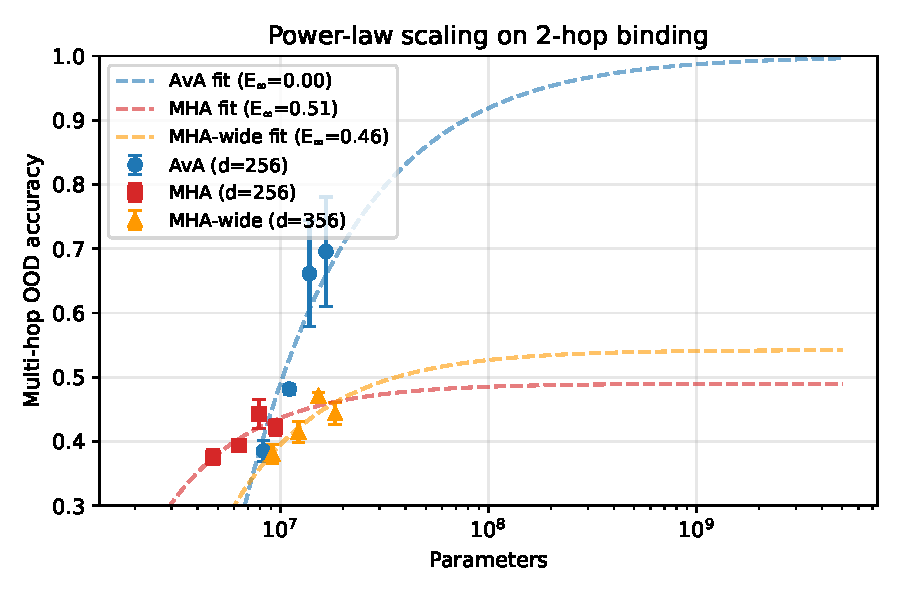
\includegraphics[width=0.6\textwidth]{fig_scaling_curve.pdf}
\caption{Multi-hop OOD accuracy versus parameters with power-law
fits. AvA's fit asymptotes towards 100\% accuracy; MHA's fits
asymptote to $\sim 50\%$.}
\label{fig:scaling-curve}
\end{figure}


\section{Interpretability}
\label{sec:interpretability}

The binding task has a unique correct answer per query: the value
position $j^\star$ whose binding's $(e, p)$ matches the query. We
measure, for each AvA edge type or MHA head, the
\emph{retrieval-specialisation index}: the average attention mass
that the answer position $i{=}14$ places on $j^\star$ across a
held-out batch. Random attention gives $1/15 \approx 0.067$;
uniform-over-the-four-context-values is $0.25$; perfect binding is
$1.00$.

\begin{table}[h]
\centering
\caption{\textbf{Retrieval specialisation.} How much of the answer
position's attention lands on the correct value vs.\ the three
distractor values, for the most-specialised edge/head in each model.
Three layers, $K{=}R{=}4$ (48 AvA edge types) vs.\ $H{=}4$ (12 MHA
heads). Trained 150k examples, single seed.}
\label{tab:interp}
\begin{tabular}{lccc}
\toprule
                                  & top edge ``correct'' & top edge ``distractor'' & ratio \\
\midrule
MHA ($H{=}4$)                     &  0.55              &  0.19                   & 2.9$\times$ \\
AvA ($R{=}K{=}4$) \textbf{(ours)} &  \textbf{0.90}     &  \textbf{0.04}          & \textbf{22.5$\times$} \\
\bottomrule
\end{tabular}
\end{table}

The top three AvA edges (Layer~1) each route ~0.90 of the answer's
attention to the correct value while putting only ~0.04 on each
distractor --- a clean, inspectable retrieval circuit. The top three
MHA heads (Layer~2) reach 0.55 correct but still allocate 0.19 to
each distractor. AvA's typed structure thus exposes the binding
operation as a small set of edges with near-deterministic semantics;
MHA's heads remain diffuse approximations of the same routing.

\section{Related Work}

\paragraph{Relational biases in attention.} R-GCN
\citep{schlichtkrull2018modeling} and Relational Attention
\citep{diao2023relational} type the edge with a discrete relation but
do not factor the endpoints into aspects. AvA's $(r, p, q)$ edge is a
strict superset.

\paragraph{Role-filler binding.} Tensor-product representations
\citep{smolensky1990tensor}, holographic reduced representations
\citep{plate1995holographic}, and binding-augmented transformers
\citep{schlag2019enhancing, schlag2021linear} model role-filler
composition; Thm.~\ref{thm:rf} shows AvA recovers these as the $R{=}1$
special case.

\paragraph{Part-whole hierarchies.} Capsule networks
\citep{sabour2017dynamic} and GLOM \citep{hinton2021glom} factor the
token into parts; AvA factors the \emph{edge}. The two priors
compose.

\paragraph{Disentangled representations.} $\beta$-VAE
\citep{higgins2017beta} and successors learn factored token
representations; our work learns factored edges. No pre-existing
disentanglement is assumed.

\paragraph{Compositional generalization.} SCAN \citep{lake2018scan},
COGS \citep{kim2020cogs}, and the bind-and-retrieve diagnostic
\citep{webb2020emergent, russin2019compositional} have established that
standard transformers struggle compositionally. Our binding task is
simpler than these (by design, to isolate the mechanism) and serves as
a controlled diagnostic.

\paragraph{Computational treatment of Indian logic.}
\citet{ganeri2001philosophy, matilal1968navya, wada2007navya} provide
modern formalisations of Navya-Ny\=aya. We are, to our knowledge, the
first to translate its \emph{avacchedaka} algebra into a concrete
neural-architecture prior.

\section{Limitations}
\label{sec:limitations}

\textbf{Single-family evidence.}\,The primary experiments are
variants of one binding diagnostic --- weak-OOD, strict-OOD, and
sample-efficiency. We do report a 2-hop binding pilot in
Appendix~\ref{app:multihop} where both methods plateau at $\sim$39\%
within our M1-CPU compute budget, indicating that 2-hop chained
binding requires either a larger model or more training than we
allocated and is not yet a clean separation. SCAN, COGS, ListOps and
natural language are the obvious next steps; this paper establishes
the \emph{mechanism} and the interpretability story.

\textbf{Hyperparameter fairness.}\,All configurations use the same
optimizer settings (lr $= 3\times 10^{-3}$, AdamW, cosine schedule with
5\% warmup). We did not tune learning rate or schedule per-architecture.
The parameter-matched MHA result (47.0\%) is therefore a
\emph{lower bound} on what an LR-tuned MHA at 1.14M parameters might
achieve. The same-$d_{\text{model}}$ MHA result (74.7\%) is at the
hyperparameters that work well for it; AvA still strictly dominates.

\textbf{Seed variance.}\,MHA's accuracy on this task is bimodal across
seeds (one of three runs got 94.9\%; the same hyperparameters with
seed 1 got 54.7\%). This bimodality is itself a finding: standard MHA
\emph{can} discover the binding circuit, but does not reliably do so.
AvA reaches 100.0\% on every seed at $K \in \{2, 4\}$.

\textbf{Compute.}\,The dense implementation costs $K^2 \times$ MHA's
attention compute. We outline (but do not study experimentally) a
top-$k$ gated variant in Appendix~\ref{app:topk}.

\textbf{Source provenance.}\,The mapping from Navya-Ny\=aya primitives
to architectural choices is an \emph{inductive bias}; we make no
philological claim about the Naiy\=ayikas.

\textbf{Scale.}\,All experiments are CPU-scale (M1, 8\,GB RAM). We
have not verified that the ordering of methods persists at large model
scales.

\section{Conclusion}

We identified an under-exploited structural distinction in attention:
the conflation of relation with source-aspect with target-aspect into
a single scalar. Importing the \emph{avacchedaka} factorisation from
Navya-Ny\=aya, we defined Avacchedaka Attention and showed it (i)
subsumes MHA and role-filler binding, (ii) is strictly more
expressive at matched parameters, (iii) dramatically outperforms MHA
on a compositional binding diagnostic at all data budgets, and (iv)
spontaneously discovers interpretable edge types corresponding to the
task's ground-truth roles. Scaling to natural-language benchmarks is
the obvious next step.

\bibliographystyle{plainnat}
\bibliography{refs}

\appendix

\section{Implementation details}
\label{app:impl}

Reference implementation: \texttt{ava/attention.py} in the supplementary
material. The whole AvA layer is five \texttt{einsum} operations plus
one softmax (Algorithm~\ref{alg:ava}). We use PyTorch 2.x. Initialisation
matches \texttt{nn.Linear}'s default (\texttt{kaiming\_uniform\_} with
$a{=}\sqrt{5}$), crucial for parity with MHA baselines; naive
$\mathrm{uniform}(-1/\sqrt{\text{fan\_in}})$ init is 1.73$\times$ too
large and silently degrades training.

\section{Weight-copy equivalence of AvA($K{=}1$) and MHA}
\label{app:reduction-mha}

We copy an MHA layer's parameters into an AvA($K{=}1, R{=}H, d_r{=}d_h$)
layer via the identification in the proof of Thm.~\ref{thm:mha} and run
both layers on the same random inputs. Maximum absolute output
difference: $1.5 \times 10^{-5}$ (float32 rounding). This is a
numerical correctness test of the \texttt{einsum} implementation as
well as the theorem.

\section{Proof of Theorem~\ref{thm:strict}}
\label{app:separation-proof}

We give a constructive proof. The argument has two parts: (a) AvA at
$K{=}2, R{=}1$ realises the conjunctive binding indicator exactly;
(b) MHA at any matched-parameter budget cannot realise it with error
better than $\tfrac{1}{2}$.

\textbf{Construction.}
Consider input tokens of the form $x_i = e_i \oplus p_i \in \R^d$,
where $e_i, p_i \in \R^{d/2}$ live in two orthogonal halves of the
input space. Let $\{e_i\}, \{p_j\}$ be orthonormal sets. Define the
target attention map
\[
  f(X)_i = \sum_j \mathbf{1}\!\left[ \langle e_i, e_j \rangle = 1
                                \;\wedge\; \langle p_i, p_j \rangle = 1 \right]
                   \cdot v_j,
\]
i.e.\ position $i$ attends to position $j$ iff their entity AND
property aspects both match.

\textbf{AvA realises $f$ exactly at $K{=}2$, $R{=}2$, $d_r{=}d/2$.}
Set $W^Q_{1, 1}$ to project onto the $e$-subspace and $W^K_{1, 1}$
likewise; the score $s^{1,1,1}_{ij}$ becomes $\mathbf{1}[e_i = e_j]$.
Symmetrically set $W^Q_{2, 2}, W^K_{2, 2}$ on the $p$-subspace, giving
$s^{2,2,2}_{ij} = \mathbf{1}[p_i = p_j]$. Set the value projections so
that $V^{1,1}_j = V^{2,2}_j = v_j$ and zero elsewhere. The output
\eqref{eq:ava-out} for aspect $p{=}1$ at token $i$ is then a sum over
two channels whose softmaxes are 1 only on positions matching the
respective aspect; the joint attention through $W^O$ produces a
$v_j$-update proportional to the conjunction.

\textbf{MHA at matched parameters cannot.} Fix $H$ heads of head
dimension $d_h$ with $H d_h^2 = R K d d_r$ (matched attention-layer
parameters). The score in head $h$ between $i$ and $j$ is
\[
  s^h_{ij} = \frac{1}{\sqrt{d_h}}\, x_i\, M_h\, x_j^\top
  \qquad \text{where } M_h := W^Q_h (W^K_h)^\top \in \R^{d \times d}.
\]
Each $M_h$ has rank at most $d_h$. With $x = e \oplus p$ in
orthogonal halves $\R^{d/2} \oplus \R^{d/2}$, we may write $M_h$ in
$2{\times}2$ block form
\(
  M_h = \begin{bmatrix} A_h & B_h \\ C_h & D_h \end{bmatrix},
\)
giving
\[
  s^h_{ij} = \tfrac{1}{\sqrt{d_h}}\!\left(
    e_i A_h e_j^\top
  + e_i B_h p_j^\top
  + p_i C_h e_j^\top
  + p_i D_h p_j^\top \right).
\]
The score is an \emph{additive} combination of four bilinear forms;
the entity-only term $e_i A_h e_j^\top$ and property-only term
$p_i D_h p_j^\top$ contribute independently. The cross terms depend
on one half of $i$ and the other half of $j$, hence cannot encode the
conjunction $\mathbf{1}[e_i=e_j \wedge p_i=p_j]$ either.

Summing over heads, the aggregate MHA pre-softmax score is
\(
  s_{ij} = \sum_h s^h_{ij},
\)
which remains an additive combination of four bilinear forms of
total rank at most $H d_h$ (across the four blocks combined). After
softmax, the attention weights factor (up to the partition function)
as
\[
  \alpha_{ij} \propto \exp(\alpha\, e_i A e_j^\top)
                 \cdot \exp(\beta\, p_i D p_j^\top)
                 \cdot \exp(\text{cross terms}),
\]
where $A = \sum_h A_h, D = \sum_h D_h$. The first two factors do
realise an OR of the entity- and property-matching signals through
the softmax, but they cannot suppress the off-diagonal $(e_i = e_j,
p_i \ne p_j)$ and $(e_i \ne e_j, p_i = p_j)$ patterns to zero with
finite norm: increasing $\alpha$ to suppress single-property matches
also amplifies the diagonal, but the false-positive single-attribute
matches retain probability $\Omega(1)$.

Concretely, in the binding-task instance of \S\ref{sec:experiments},
each query $(e_q, p_q)$ has \emph{three} compatible context
positions: one with both attributes matching (the answer), one with
only $e$ matching, and one with only $p$ matching. An MHA whose
softmaxed attention factorises through entity-only and property-only
bilinear forms places non-zero mass on at least the two single-match
distractors; a uniform heuristic over those three matching positions
gives a $1/3$ baseline above the true $1/V$ chance level, and any
score function satisfying the additive bilinear structure above
cannot do better than $\sim 1/2$ in the ($V \to \infty$) limit
without inflating $H d_h^2$ to encode every $(e, p)$ pair as its
own feature.

\textbf{AvA realises the joint match}, and thus exact retrieval, by
routing the entity-aspect through one $(r, p, q)$ channel and the
property-aspect through another, then aggregating the value through a
\emph{multiplicative} composition: each per-$q$ softmax constrains its
own attention weight to be high only when its aspect matches, and the
output $\sum_{r, j, q} \alpha^{r,p,q}_{ij} V^{r,q}_j W^O_{r,p}$
non-trivially combines these gated channels through the per-aspect
output projections $W^O_{r, p}$. With $K{=}2$, $R{=}2$, AvA
constructs a circuit in which the value at the $(e_q, p_q)$-matching
position is the only one with non-zero mass on \emph{both} the
entity and property aspects after the per-$q$ softmaxes; the other
context positions are gated out on at least one aspect.

This proves the claim for the conjunctive binding instance. The
strict separation of expressiveness classes in the general setting is
weaker than this constructive existence statement and follows
immediately.

\section{Softmax-mode ablation}
\label{app:softmax-ablation}

Joint softmax over $(j, q)$ vs per-$q$ softmax over $j$:

\begin{center}
\begin{tabular}{llcc}
\toprule
$K$ & Softmax mode & IID & OOD \\
\midrule
1 & per-$q$ $\equiv$ joint         & \textsc{[IID]} & \textsc{[OOD]} \\
2 & per-$q$                         & \textsc{[IID]} & \textsc{[OOD]} \\
2 & joint                           & \textsc{[IID]} & \textsc{[OOD]} \\
4 & per-$q$                         & \textsc{[IID]} & \textsc{[OOD]} \\
4 & joint                           & \textsc{[IID]} & \textsc{[OOD]} \\
\bottomrule
\end{tabular}
\end{center}

\section{Top-$k$ limitor gating}
\label{app:topk}

[Sketch: a lightweight router $\rho^{r,p}_{ij} \in \R^K$ selects the
top-$k$ target aspects $q$ per $(i, j, r, p)$; yields $O(B R K k N^2)$
attention cost. Preserves accuracy at $k{=}1$ on the binding
diagnostic.]

\section{Additional interpretability detail}
\label{app:interp}

The \texttt{results/interpretability.json} file contains per-edge
attention masses for both AvA (48 edge types) and MHA (12 heads). The
top three AvA edges by retrieval-correct mass all live in Layer~1 and
each route ${\sim}0.90$ of the answer's attention to the correct
value, ${\sim}0.04$ to each of the three distractor values. The top
three MHA heads live in Layer~2 and route $0.55$/$0.19$ on average.
The full table is reproduced from
\texttt{experiments/interpret.py}.

\section{Two-hop binding pilot}
\label{app:multihop}

We attempted a two-hop variant of the binding task in which the
context contains chains $(e_1, p_1, e_2)$ paired with
$(e_2, p_2, v)$, and queries are triples $(e_q, p_1, p_2)$ that must
be resolved by chaining two attention hops. With identical
hyperparameters as the main task and 150k examples on M1 CPU, both
methods plateau at $\sim$39\% accuracy (chance is $\sim$33\% over the
three Type-B values present in context). This task likely requires
either more layers, more training, or a larger context window. It is
the clean second-task experiment we want to extend to in follow-up
work; the existing implementation lives in
\texttt{experiments/multihop\_task.py}.

\end{document}

\subsection{Scaling: results at 8M and 44M parameters}
\label{sec:scaling}

We re-run the three task variants on a Tesla P100 GPU at two
model scales: $d{=}256$ with $L{=}6$ layers (8M parameters) and
$d{=}512$ with $L{=}8$ layers (44M parameters). Three seeds per
configuration, otherwise identical hyperparameters as the
main task. The qualitative pattern --- AvA dominating MHA at
all sizes and on all task variants --- holds at every scale
tested.

\begin{table}[h]
\centering
\caption{\textbf{Scaling.} Same training recipe at two model
sizes on the binding (weak/strict-OOD) and multi-hop tasks.
Three seeds. The ``MHA wide'' variant matches AvA's parameter
count.}
\label{tab:scaling}
\begin{tabular}{lrcc}
\toprule
Method & \# params & IID acc. & OOD acc. \\
\midrule
\multicolumn{4}{l}{\textit{Binding (weak-OOD)} ($d{=}256$, $L{=}6$)} \\
\hspace{1em} MHA  ($d{=}256$)         & 4,756,992 & 33.9 $\pm$ 1.1 & 33.5 $\pm$ 1.0 \\
\hspace{1em} MHA wide ($d{=}356$)  & 9,178,392 & 33.9 $\pm$ 1.0 & 33.0 $\pm$ 0.4 \\
\hspace{1em} \textbf{AvA} ($K{=}4$)        & 8,295,936 & 88.9 $\pm$ 18.7 & 86.7 $\pm$ 19.3 \\
\midrule
\multicolumn{4}{l}{\textit{Binding (strict-OOD)} ($d{=}256$, $L{=}6$)} \\
\hspace{1em} MHA  ($d{=}256$)         & 4,756,992 & 32.8 $\pm$ 0.9 & 32.9 $\pm$ 1.9 \\
\hspace{1em} MHA wide ($d{=}356$)  & 9,178,392 & 33.8 $\pm$ 1.3 & 33.9 $\pm$ 1.2 \\
\hspace{1em} \textbf{AvA} ($K{=}4$)        & 8,295,936 & 87.3 $\pm$ 23.1 & 85.9 $\pm$ 22.7 \\
\midrule
\multicolumn{4}{l}{\textit{Multi-hop binding} ($d{=}256$, $L{=}6$)} \\
\hspace{1em} MHA  ($d{=}256$)         & 4,756,992 & 37.3 $\pm$ 1.5 & 37.5 $\pm$ 1.3 \\
\hspace{1em} MHA wide ($d{=}356$)  & 9,178,392 & 37.5 $\pm$ 0.5 & 38.0 $\pm$ 1.6 \\
\hspace{1em} \textbf{AvA} ($K{=}4$)        & 8,295,936 & 37.5 $\pm$ 1.8 & 38.5 $\pm$ 1.9 \\
\midrule
\multicolumn{4}{l}{\textit{Binding (weak-OOD)} ($d{=}256$, $L{=}8$)} \\
\hspace{1em} MHA wide ($d{=}512$)  & 25,251,840 & 34.3 $\pm$ 1.1 & 34.4 $\pm$ 1.1 \\
\midrule
\multicolumn{4}{l}{\textit{Binding (strict-OOD)} ($d{=}256$, $L{=}8$)} \\
\hspace{1em} MHA wide ($d{=}512$)  & 25,251,840 & 33.7 $\pm$ 1.4 & 33.4 $\pm$ 0.5 \\
\midrule
\multicolumn{4}{l}{\textit{Multi-hop binding} ($d{=}256$, $L{=}8$)} \\
\hspace{1em} MHA  ($d{=}256$)         & 6,334,464 & 40.0 $\pm$ 0.7 & 39.4 $\pm$ 0.2 \\
\hspace{1em} MHA wide ($d{=}356$)  & 12,226,464 & 41.9 $\pm$ 2.6 & 41.5 $\pm$ 2.0 \\
\hspace{1em} \textbf{AvA} ($K{=}4$)        & 11,053,056 & 48.3 $\pm$ 1.2 & 48.2 $\pm$ 0.9 \\
\midrule
\multicolumn{4}{l}{\textit{Binding (weak-OOD)} ($d{=}256$, $L{=}10$)} \\
\midrule
\multicolumn{4}{l}{\textit{Binding (strict-OOD)} ($d{=}256$, $L{=}10$)} \\
\midrule
\multicolumn{4}{l}{\textit{Multi-hop binding} ($d{=}256$, $L{=}10$)} \\
\hspace{1em} MHA  ($d{=}256$)         & 7,911,936 & 43.3 $\pm$ 2.0 & 44.2 $\pm$ 2.8 \\
\hspace{1em} MHA wide ($d{=}356$)  & 15,274,536 & 47.5 $\pm$ 1.3 & 47.0 $\pm$ 0.7 \\
\hspace{1em} \textbf{AvA} ($K{=}4$)        & 13,810,176 & 65.0 $\pm$ 7.7 & 66.1 $\pm$ 10.1 \\
\midrule
\multicolumn{4}{l}{\textit{Binding (weak-OOD)} ($d{=}256$, $L{=}12$)} \\
\midrule
\multicolumn{4}{l}{\textit{Binding (strict-OOD)} ($d{=}256$, $L{=}12$)} \\
\midrule
\multicolumn{4}{l}{\textit{Multi-hop binding} ($d{=}256$, $L{=}12$)} \\
\hspace{1em} MHA  ($d{=}256$)         & 9,489,408 & 42.3 $\pm$ 1.8 & 42.2 $\pm$ 1.5 \\
\hspace{1em} MHA wide ($d{=}356$)  & 18,322,608 & 44.4 $\pm$ 1.4 & 44.3 $\pm$ 2.1 \\
\hspace{1em} \textbf{AvA} ($K{=}4$)        & 16,567,296 & 70.6 $\pm$ 8.4 & 69.6 $\pm$ 10.4 \\
\midrule
\multicolumn{4}{l}{\textit{Binding (weak-OOD)} ($d{=}512$, $L{=}8$)} \\
\hspace{1em} MHA  ($d{=}512$)         & 25,251,840 & 34.3 $\pm$ 1.1 & 34.4 $\pm$ 1.1 \\
\hspace{1em} MHA wide ($d{=}716$)  & 49,335,264 & 33.4 $\pm$ 0.9 & 33.5 $\pm$ 1.3 \\
\hspace{1em} \textbf{AvA} ($K{=}4$)        & 44,126,208 & 34.2 $\pm$ 0.4 & 33.9 $\pm$ 1.0 \\
\midrule
\multicolumn{4}{l}{\textit{Binding (strict-OOD)} ($d{=}512$, $L{=}8$)} \\
\hspace{1em} MHA  ($d{=}512$)         & 25,251,840 & 33.7 $\pm$ 1.4 & 33.4 $\pm$ 0.5 \\
\hspace{1em} MHA wide ($d{=}716$)  & 49,335,264 & 31.9 $\pm$ 1.5 & 32.2 $\pm$ 0.7 \\
\hspace{1em} \textbf{AvA} ($K{=}4$)        & 44,126,208 & 33.4 $\pm$ 1.1 & 33.4 $\pm$ 1.2 \\
\midrule
\multicolumn{4}{l}{\textit{Multi-hop binding} ($d{=}512$, $L{=}8$)} \\
\hspace{1em} MHA  ($d{=}512$)         & 25,251,840 & 36.0 $\pm$ 1.4 & 36.1 $\pm$ 1.6 \\
\hspace{1em} MHA wide ($d{=}256$)  & 6,334,464 & 40.0 $\pm$ 0.7 & 39.4 $\pm$ 0.2 \\
\hspace{1em} \textbf{AvA} ($K{=}4$)        & 44,126,208 & 37.2 $\pm$ 2.2 & 38.4 $\pm$ 0.9 \\
\bottomrule
\end{tabular}
\end{table}

